% =========================================================================
\chapter{From days to rows: the 57 predictors}
\label{ch:rows}
% =========================================================================

\section{What a row is}
The classifier reads a \textbf{table}. One \textbf{row} is one cell on one day (a \emph{cell-day}); its columns are the
\textbf{predictors} (also called features or inputs) plus the label. A year gives about $529\times365\approx193{,}000$
rows. The classifier does not read a sequence of days, so the past must be written into the columns of the row: that is
why there are columns for yesterday, the day before, and summaries of the last weeks.

\begin{figure}[H]
\centering
\begin{tikzpicture}[x=0.42cm,y=0.5cm,
  dbox/.style={draw=black!50,fill=#1,minimum height=0.5cm,minimum width=0.42cm,inner sep=0}]
\foreach \i in {0,...,29} { \node[dbox=black!4] at (\i,0) {}; }
\foreach \i in {27,28} { \node[dbox=blue!18] at (\i,0) {}; }
\node[dbox=orange!35] at (29,0) {};
\node[dbox=red!25,draw=red!60!black] at (31.2,0) {};
\node[font=\scriptsize,below] at (0,-0.4) {$D\!-\!29$};
\node[font=\scriptsize,below] at (16,-0.4) {$D\!-\!13$};
\node[font=\scriptsize,below] at (23,-0.4) {$D\!-\!6$};
\node[font=\scriptsize,below] at (27,-0.4) {$D\!-\!2$};
\node[font=\scriptsize,below] at (29,-0.4) {today $D$};
\node[font=\scriptsize,below] at (31.2,-0.4) {$D\!+\!1$};
\draw[decorate,decoration={brace,amplitude=4pt},thick] (-0.5,0.6) -- (29.5,0.6) node[midway,above=4pt,font=\scriptsize]{last 30 / 14 / 7 days: summaries (16 numbers)};
\draw[decorate,decoration={brace,amplitude=4pt,mirror},thick] (26.5,-1.6) -- (29.5,-1.6) node[midway,below=4pt,font=\scriptsize,align=center]{last 3 days: 9 values each\\$=27$ numbers};
\node[font=\scriptsize,align=center,red!50!black] at (31.2,1.8) {label};
\draw[-{Stealth[length=2mm]},thick] (29.6,0) -- (30.6,0);
\end{tikzpicture}
\caption{The days one row looks at. Only days up to today are used; nothing from tomorrow except the label.}
\end{figure}

\section{The five groups of predictors}
\begin{table}[H]
\centering
\caption{The 57 predictors grouped. The full list with units is Table 6 of the report.}
\footnotesize
\begin{tabularx}{\textwidth}{>{\raggedright\arraybackslash}p{3.3cm}c>{\raggedright\arraybackslash}X}
\toprule
\textbf{Group} & \textbf{How many} & \textbf{What is in it}\\
\midrule
A. Place & 4 & latitude, longitude, mean elevation, mean slope\\
B. Last three days & 27 & 9 daily values (max, min and mean temperature, dewpoint, humidity, pressure, sunshine, soil
  water, rain) for today, yesterday and the day before: $9\times3$\\
C. Today vs.\ normal & 2 & today's maximum and minimum temperature minus their normal\\
D. Last 1--4 weeks & 16 & average warmth over 7/14/30 days (5), length of the current warm spell, days since the last
  extreme, number of extremes in 30 days, rain over 7/30 days (2), soil water over 14/30 days (2), soil drying over 14
  days, average dewpoint and sunshine over 7 days (2), pressure change over 3 days\\
E. Gap to tomorrow's threshold & 8 & how far the last three days' maximum temperatures are from tomorrow's threshold, in
  $^\circ$C (3) and in units of the cell's variability (3), whether the gap is closing, and today's change in
  temperature\\
\midrule
\textbf{Total} & \textbf{57} & $4+27+2+16+8$\\
\bottomrule
\end{tabularx}
\end{table}

\begin{example}[Reading one row: Mandi, tomorrow]
To predict whether tomorrow will be extreme at the cell containing Mandi, the row contains: where the cell is and how
high it is (A); today's, yesterday's and the day before's weather there (B); whether today is warmer than usual for the
date (C); whether the last month has been hot and dry, how long the warm spell has lasted, and when the last extreme was
(D); and how close today's temperature already is to Mandi's own threshold for tomorrow's season (E). The model answers
with a probability that tomorrow is extreme.
\end{example}

\textbf{Why group E matters most:} if today is already only 0.5\,$^\circ$C below the threshold and warming, tomorrow
crossing it is likely. LightGBM is told that a smaller gap can never mean a \emph{lower} risk (a ``monotone
constraint'', Chapter~\ref{ch:clf}).

\section{Training, validation and test: splitting by time}
\begin{figure}[H]
\centering
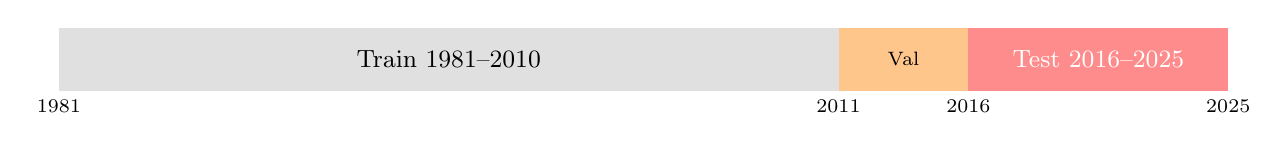
\begin{tikzpicture}[x=0.33cm]
\fill[black!12] (0,0) rectangle (30,0.8); \node[font=\small] at (15,0.4) {Train 1981--2010};
\fill[orange!45] (30,0) rectangle (35,0.8); \node[font=\scriptsize] at (32.5,0.4) {Val};
\fill[red!45] (35,0) rectangle (45,0.8); \node[font=\small,white] at (40,0.4) {Test 2016--2025};
\foreach \x/\y in {0/1981,30/2011,35/2016,45/2025} \node[font=\scriptsize,below] at (\x,0) {\y};
\end{tikzpicture}
\caption{The data are split by year, never at random.}
\end{figure}

\begin{center}
\footnotesize
\begin{tabular}{llrrl}
\toprule
\textbf{Part} & \textbf{Years} & \textbf{Rows} & \textbf{Extreme rows} & \textbf{Used for}\\
\midrule
Train & 1981--2010 & 2{,}889{,}927 & 29{,}604 (1.02\%) & fitting the classifier and the generators\\
Validation & 2011--2015 & 965{,}954 & 9{,}626 (1.00\%) & every choice (when to stop, warning cut-off)\\
Test & 2016--2025 & 1{,}932{,}437 & 37{,}450 (1.94\%) & the final scores, used once\\
\bottomrule
\end{tabular}
\end{center}

\begin{itemize}
  \item \textbf{Why by time?} Weather on neighbouring days is similar. A random split would put Monday in training
        and Tuesday in test, and the model would look better than it really is (\emph{data leakage}). Splitting by
        year is how a real forecast works: learn from the past, predict the future.
  \item \textbf{Why a random half of 1981--2010?} To fit in the memory of free Google Colab. It still keeps all 29{,}604
        extreme rows of that half.
  \item \textbf{Why a validation period?} If choices were made on the test years, the test score would be too
        optimistic. Validation is a separate ``practice exam''.
\end{itemize}

\begin{sayit}
``LightGBM reads a table, so the past is flattened into 57 columns: the place, the last three days of weather, the last
one to four weeks, and how far today is from tomorrow's threshold. I split by year: train 1981--2010, choose settings
on 2011--2015, test once on 2016--2025.''
\end{sayit}
